\lhead{\emph{Evaluation}}
\chapter{Evaluation}
\label{sec:evaluation}
To study whether the implemented Spatial Music Menu could compete with a touch and vision-based music player interface, we designed and conducted an experiment where users should perform mental and physical demanding tasks while interacting with the interfaces. This aimed to simulate the "biking while interacting with a music player" scenario.

\begin{figure}[h]
	\centering
		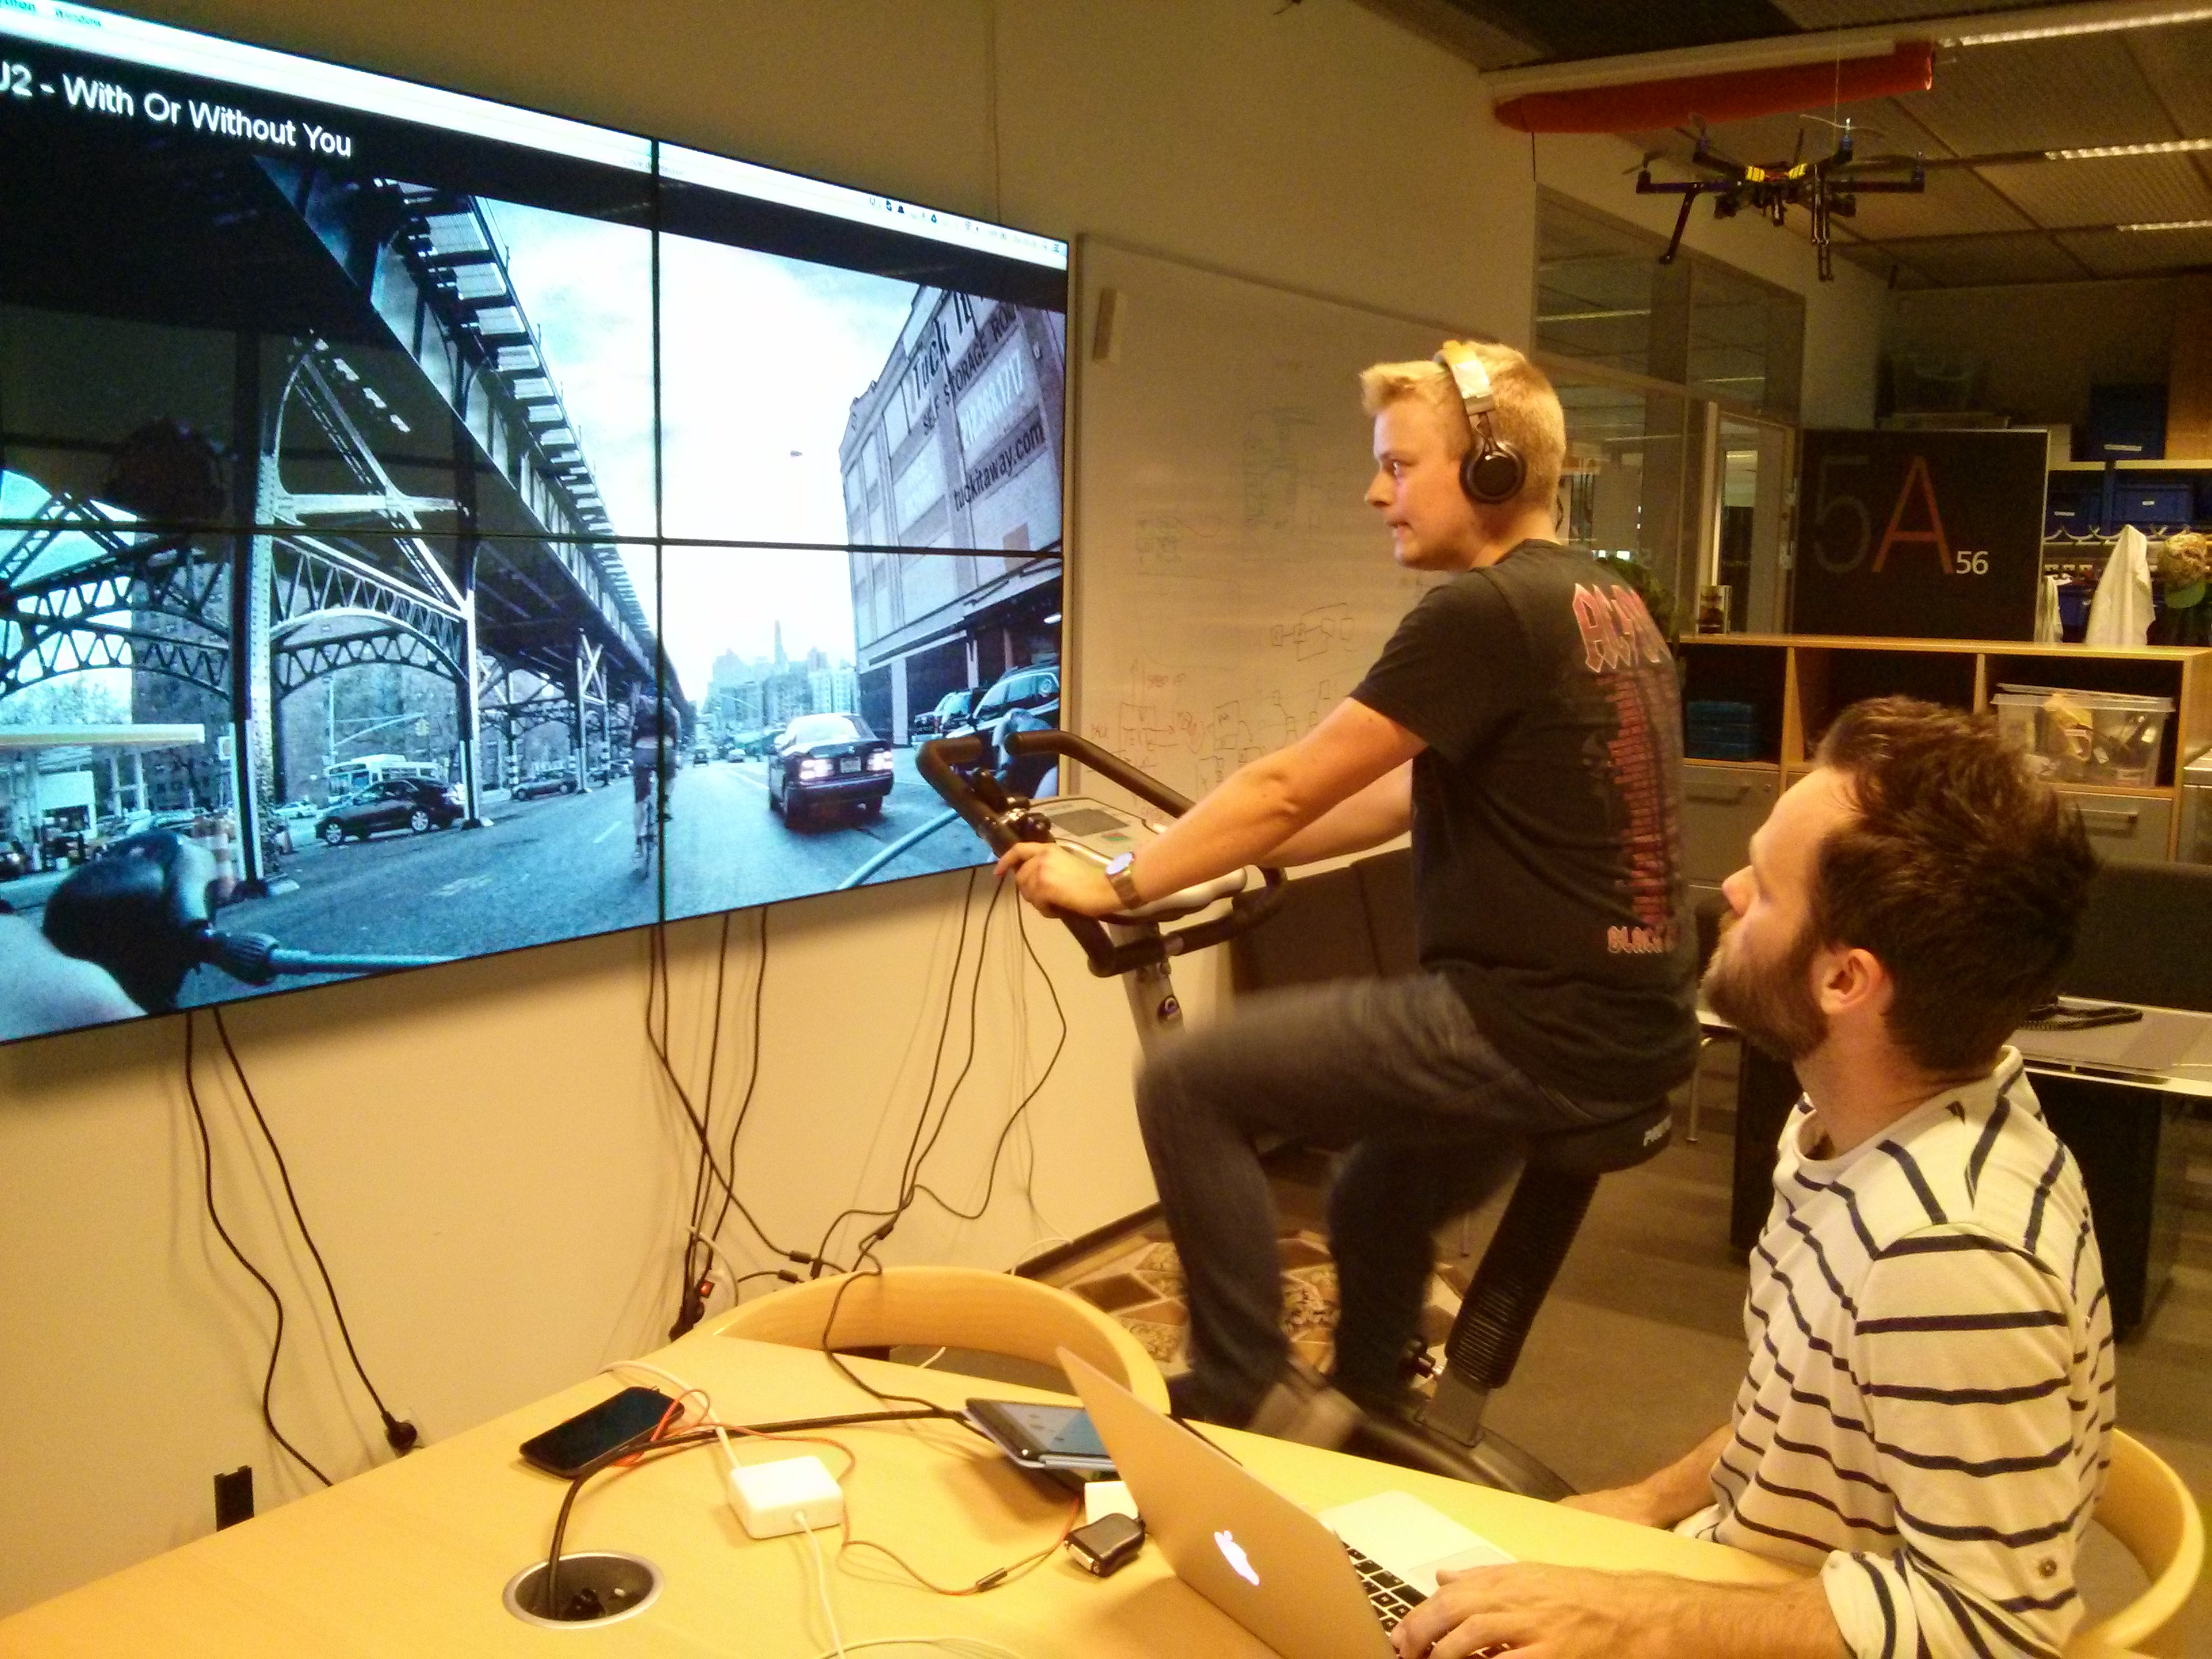
\includegraphics[width=0.7\textwidth,height=\textheight,keepaspectratio]{./Figures/evaluation_spatial.jpg}
		\rule{35em}{1pt}
	\caption[Evaluation Spatial Music Menu]{Participant performing a task using the Spatial Music Menu}
	\label{fig:evalspatial}
\end{figure}

% Scope
\textbf{Limitations and scope}

Although we in the explorative design process in \ref{sec:designsoundscape} evaluated that users could segregate 6-8 music tracks with the Spatial Music Menu, we reduced the number of tracks to 3 in this final experiment. An evaluation of the max number of simultanous playing music tracks while biking is out of this thesis scope and referred to a future study.

The participants used in the evaluation are acquaintances of us, so we are aware of the possibility that they might be biased in the sense that they want to "perform good". Throughout the experiment we tried to our best ability to be as objective as possible when explaining and instructing the systems.


\section{Experiment Design}
The experiment was designed and conducted as a controlled lab experiment. Controlled experiments are appropriate when comparing one design to another to see which is better \cite{benyon_designing_2010} and in this case we are compairing the Spatial Music Menu with a touch and vision-based music player. As the focus is on compairing and study the effects of these interfaces in an interaction in motion scenario i.e. biking, we designed an evaluation system simulating a trafficked biking scenario.

\subsection{Biking simulation}
A stationary bike was put in front of a giant screen (4 x 40 inch HD screens) that should simulate a road. To make the view as realistic as possible an image of an actual trafficked road\footnote{New York street: \url{http://timsklyarov.com/new-york-through-the-eyes-of-a-road-bicycle/}} was showed on the screen. To simulate obstacles that the user should be aware of or respond to in a real world biking scenario, 3 different shapes with random colors were displayed in random positions on the screen in a random time interval; between 0.3 and 1 second displaying the shape in 0.8 seconds. The shapes were circles, triangles and squares and the job for the person riding the bike was to detect the circles. This was done by pushing a button attached close to the users non-preferred hand on the steer, in this case a Playstation 3 joystick strapped with tape. The reason for the button placement at the non-preferred hand was, that the preferred hand should be used for navigating the touch and vision-based music player. To give the user feedback the circle was removed when detected. The screen simulation software is developed in Python 3 running on a Mac (OSX 10.9). The simulation system is illustrated in figure \ref{fig:simulationsystem}.

\begin{figure}[h]
	\centering
		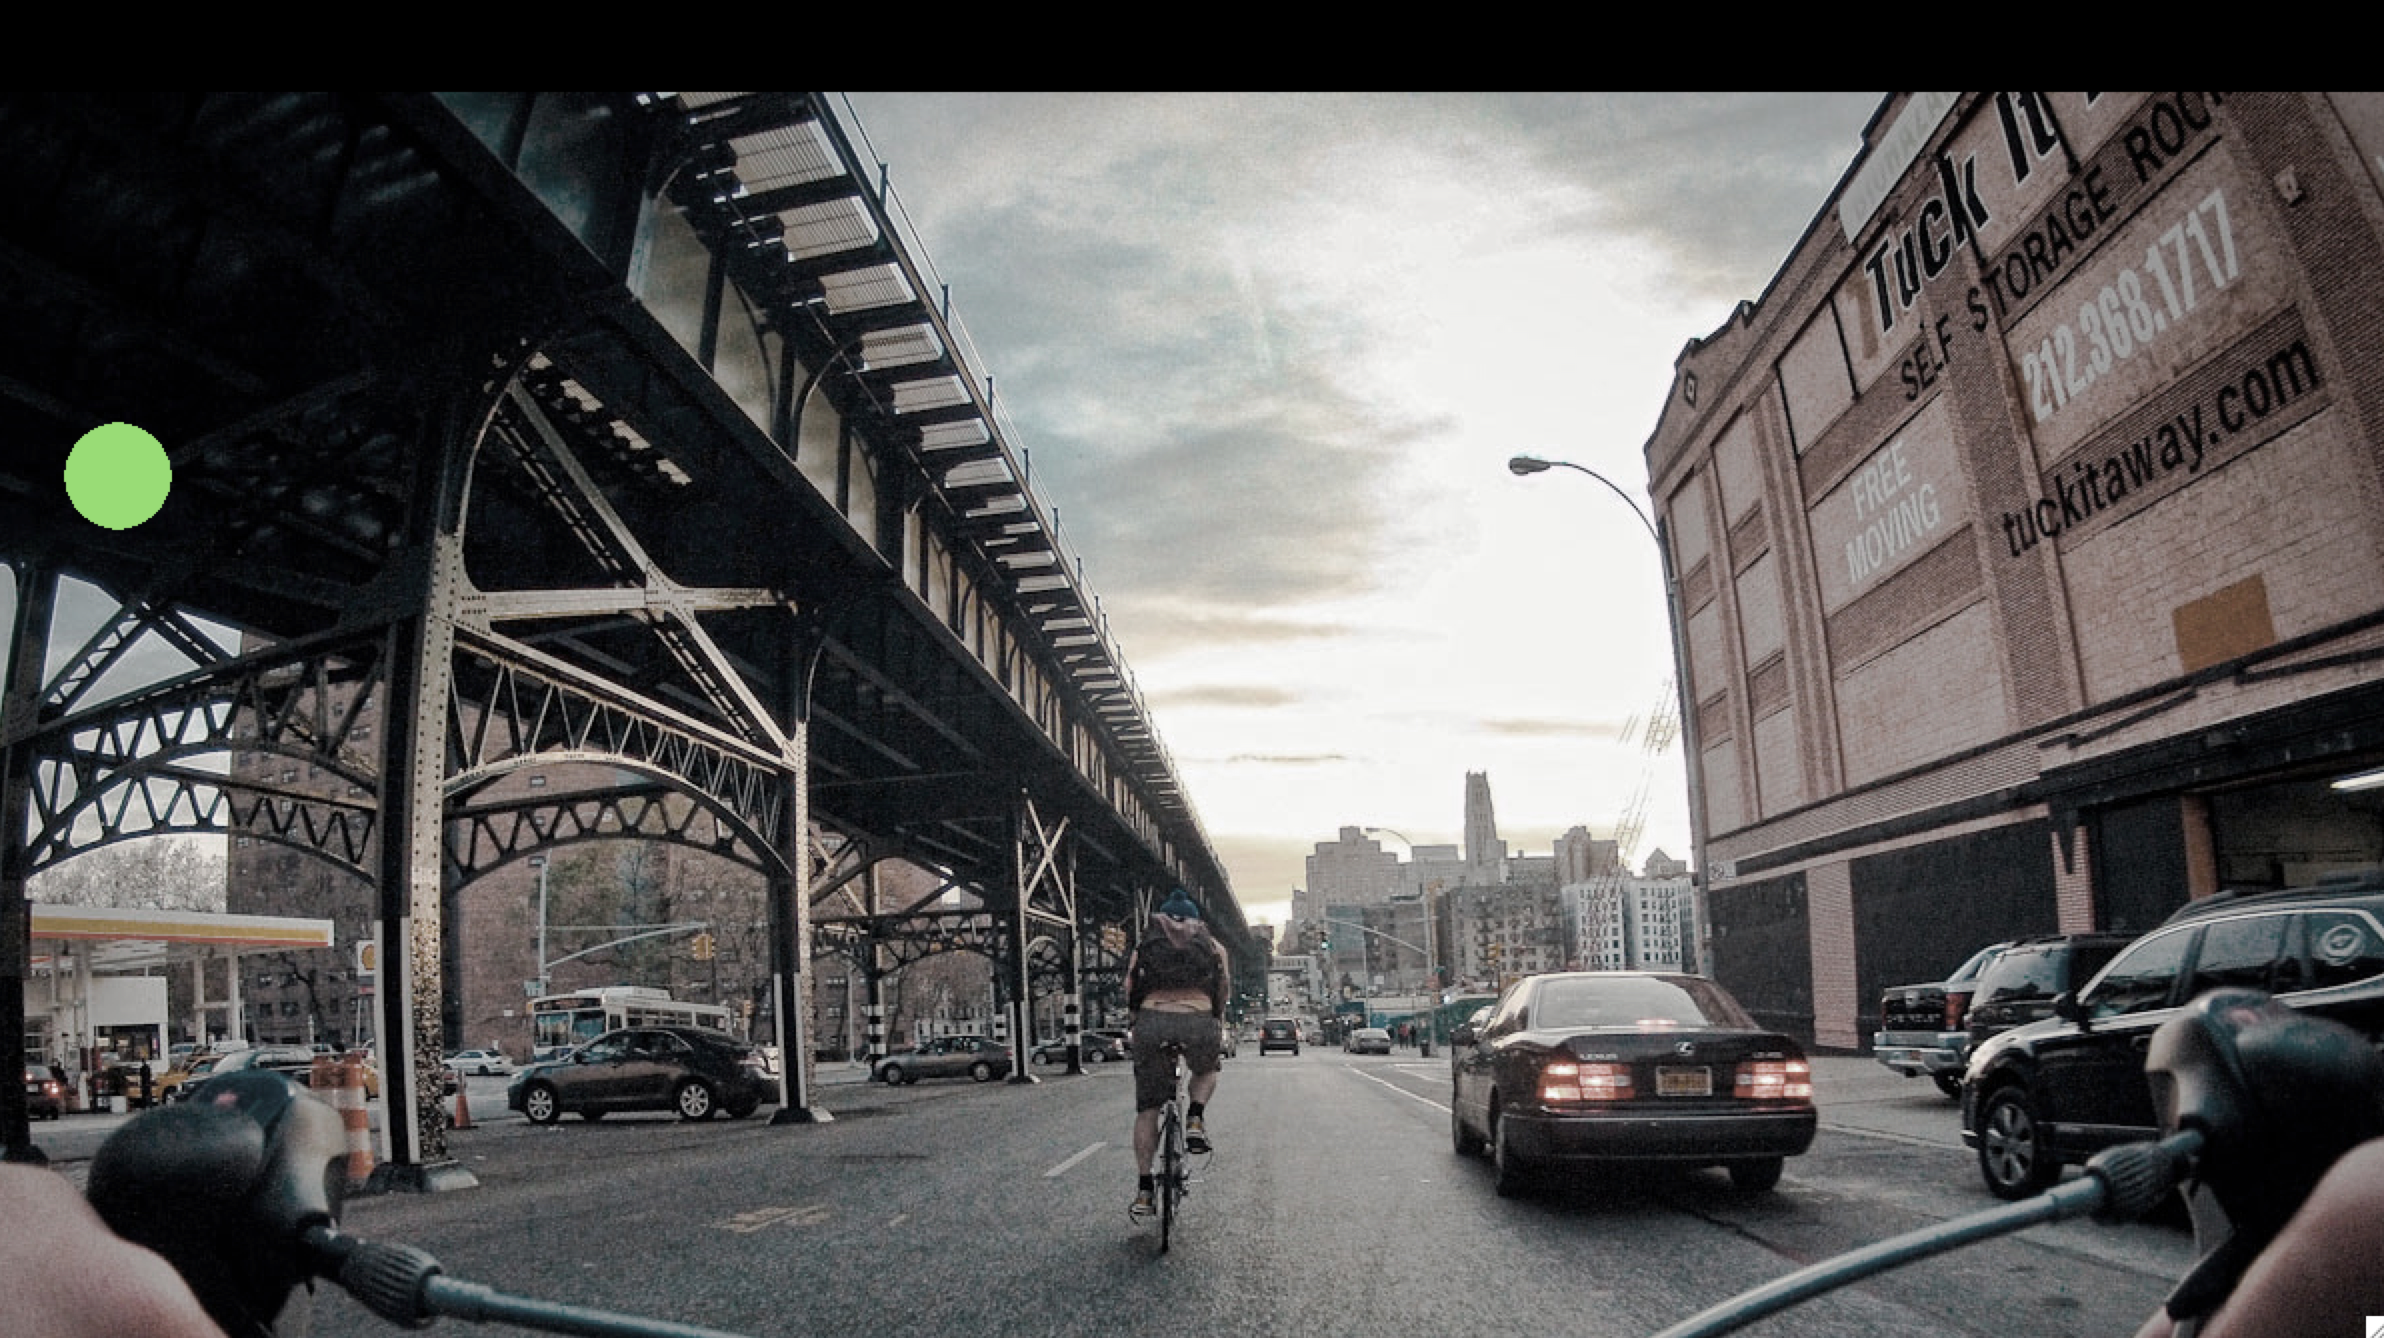
\includegraphics[width=0.6\textwidth,height=\textheight,keepaspectratio]{./Figures/simulation_system.png}
		\rule{35em}{1pt}
	\caption[Simulation screen]{The screen were to simulate a road and circles were obstacles that the user should respond to (detect) by pushing a button.}
	\label{fig:simulationsystem}
\end{figure}

\subsection{Touch and vision-based music player}
To represent a touch and vision-based music player we chose the music streaming service Deezer also used in the implementation (\ref{sec:implementationmusic}). Their Android application\footnote{\url{https://play.google.com/store/apps/details?id=deezer.android.app}} was installed on a Google Galaxy Nexus running Android 4.3. The same headset as for the Spatial Music Menu was used but this time connected through a wire.

\subsection{Hypotheses}
\label{sec:evaluationhypothesis}
Based on the related research theory and work laying ground for the design choices of the Spatial Music Menu, we derived the following hypotheses for the experiment:

\begin{description}
\item[Hypothesis 1:] The users ability to detect circles while executing tasks in the biking simulation will increase with the Spatial Music Menu interface compaired to the touch and vision-based music player interface.
\end{description}

\begin{description}
\item[Hypothesis 2:] The users performance when executing tasks in the biking simulation using the Spatial Music Menu can compete with the touch and vision-based music player interface in terms of general usability (workload) and task completion time.
\end{description}


\section{Method}
This section describes the different methods used for conducting the experiment.

\subsection{Participants}
5 persons (all male) were chosen for the evaluation. They all have in common that they listens to music while biking regularly. The participants had an average age of 30 years.

\subsection{System task}
Besides the task of detecting circles on the simulation screen the participants were given some tasks that refer to the system usage. Such a task is basically defined as a music track in which the user should navigate to. The music track (artist - title) is shown on the top left of the screen and when it does the user should start the navigation task. So in the case of the Spatial Music Menu the user should activate the menu by pushing the right button on the headset and explore and select the tracks with head gestures. If the user selects a wrong album or track the menu must be activated again (going to the HOME state). In the case of the Deezer music application the user must pick the device from a pocket, activate/unlock screen, navigate to the music track, deactivate screen and put the device back in the pocket.

As we wanted to compaire the two systems the menu structure needed to be aligned as much as possible. Figure \ref{fig:menustates} shows how the states (HOME and ALBUM) in the two different menus corresponds to each other.

\begin{figure}[t]
	\centering
		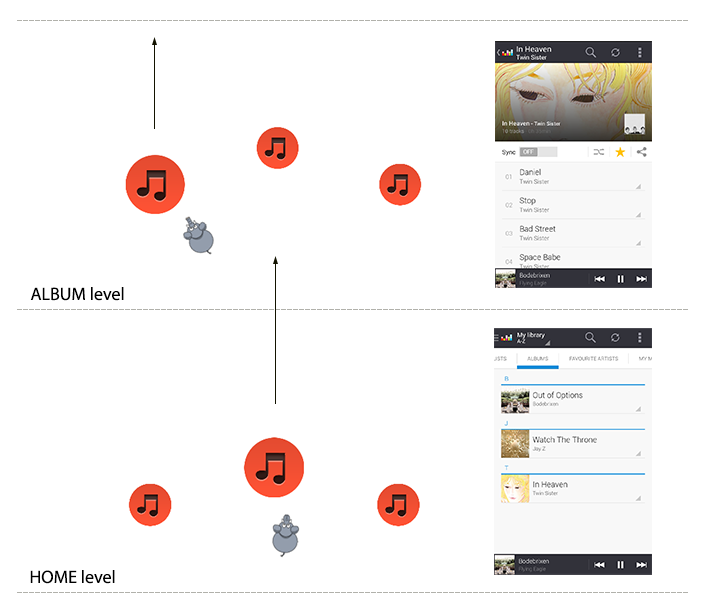
\includegraphics[width=0.9\textwidth,height=\textheight,keepaspectratio]{./Figures/menustates.png}
		\rule{35em}{1pt}
	\caption[Menu states comparison]{The HOME and ALBUM menu states definitions for each system.}
	\label{fig:menustates}
\end{figure}

The Deezer interface could imply an extra challenge in the ALBUM level, in that the entire album is showing on the screen compaired with the Spatial Music Menu where only 3 tracks appear per level. As an attempt to justify this we created an extra challenge in shuffling the 3 tracks on both levels in the Spatial Music Menu preventing the user to create a virtual map of the tracks. This would also enforce the spatialisation effect if users were still able to select and explore tracks efficiently.

\subsection{Procedure}
% Before test
As an intitial requirement for the experiment the participants had to select some of their favourite music tracks to be used in the systems - more specifically they had to choose 3 tracks from the same album for 3 different artists i.e. 9 tracks in total. The users were told that the music tracks should be very familiar e.g. hearing the song should trigger the artist name and song title.

Before starting the experiment the user were instructed in how the Spatial Music Menu works i.e. which head gestures to use for navigating and how the menu structure looks. They then got a chance to try out the system both standing still and while riding the stationary bike. In the standing still scenario the user was allowed to look at the menu envisioned on the iPad screen to get a sense of the menu structure and interaction feedback.

When the user felt ready the experiment started. The user started riding the bike and detecting the circles on the screen while listening to a chosen music track. While the gyroscope in the Intelligent Headset requires up to 10 seconds on application startup to calibrate we waited 10 seconds and then calibrated it again only this time with our system (aligning the center of the menu, described in \ref{sec:implementationviewsandcontrollers}). During the experiment 9 different system tasks were given to the user and when a task was done the user raised the right hand and a timestamp was registered in the simulation system (simple push of a button by the observer). The user were to detect circles at the same time throughout the experiment.

A user conducted this procedure for both the Spatial Music Menu and the Deezer music application and the order of which system was evaluated first were split so that 3 participants started with the Spatial Music Menu and 2 started with the Deezer application. Figure \ref{fig:evalspatial} and \ref{fig:evalnormal} shows a user performing a task using the Spatial Music Menu and the Deezer music player respectively.

\begin{figure}[t]
	\centering
		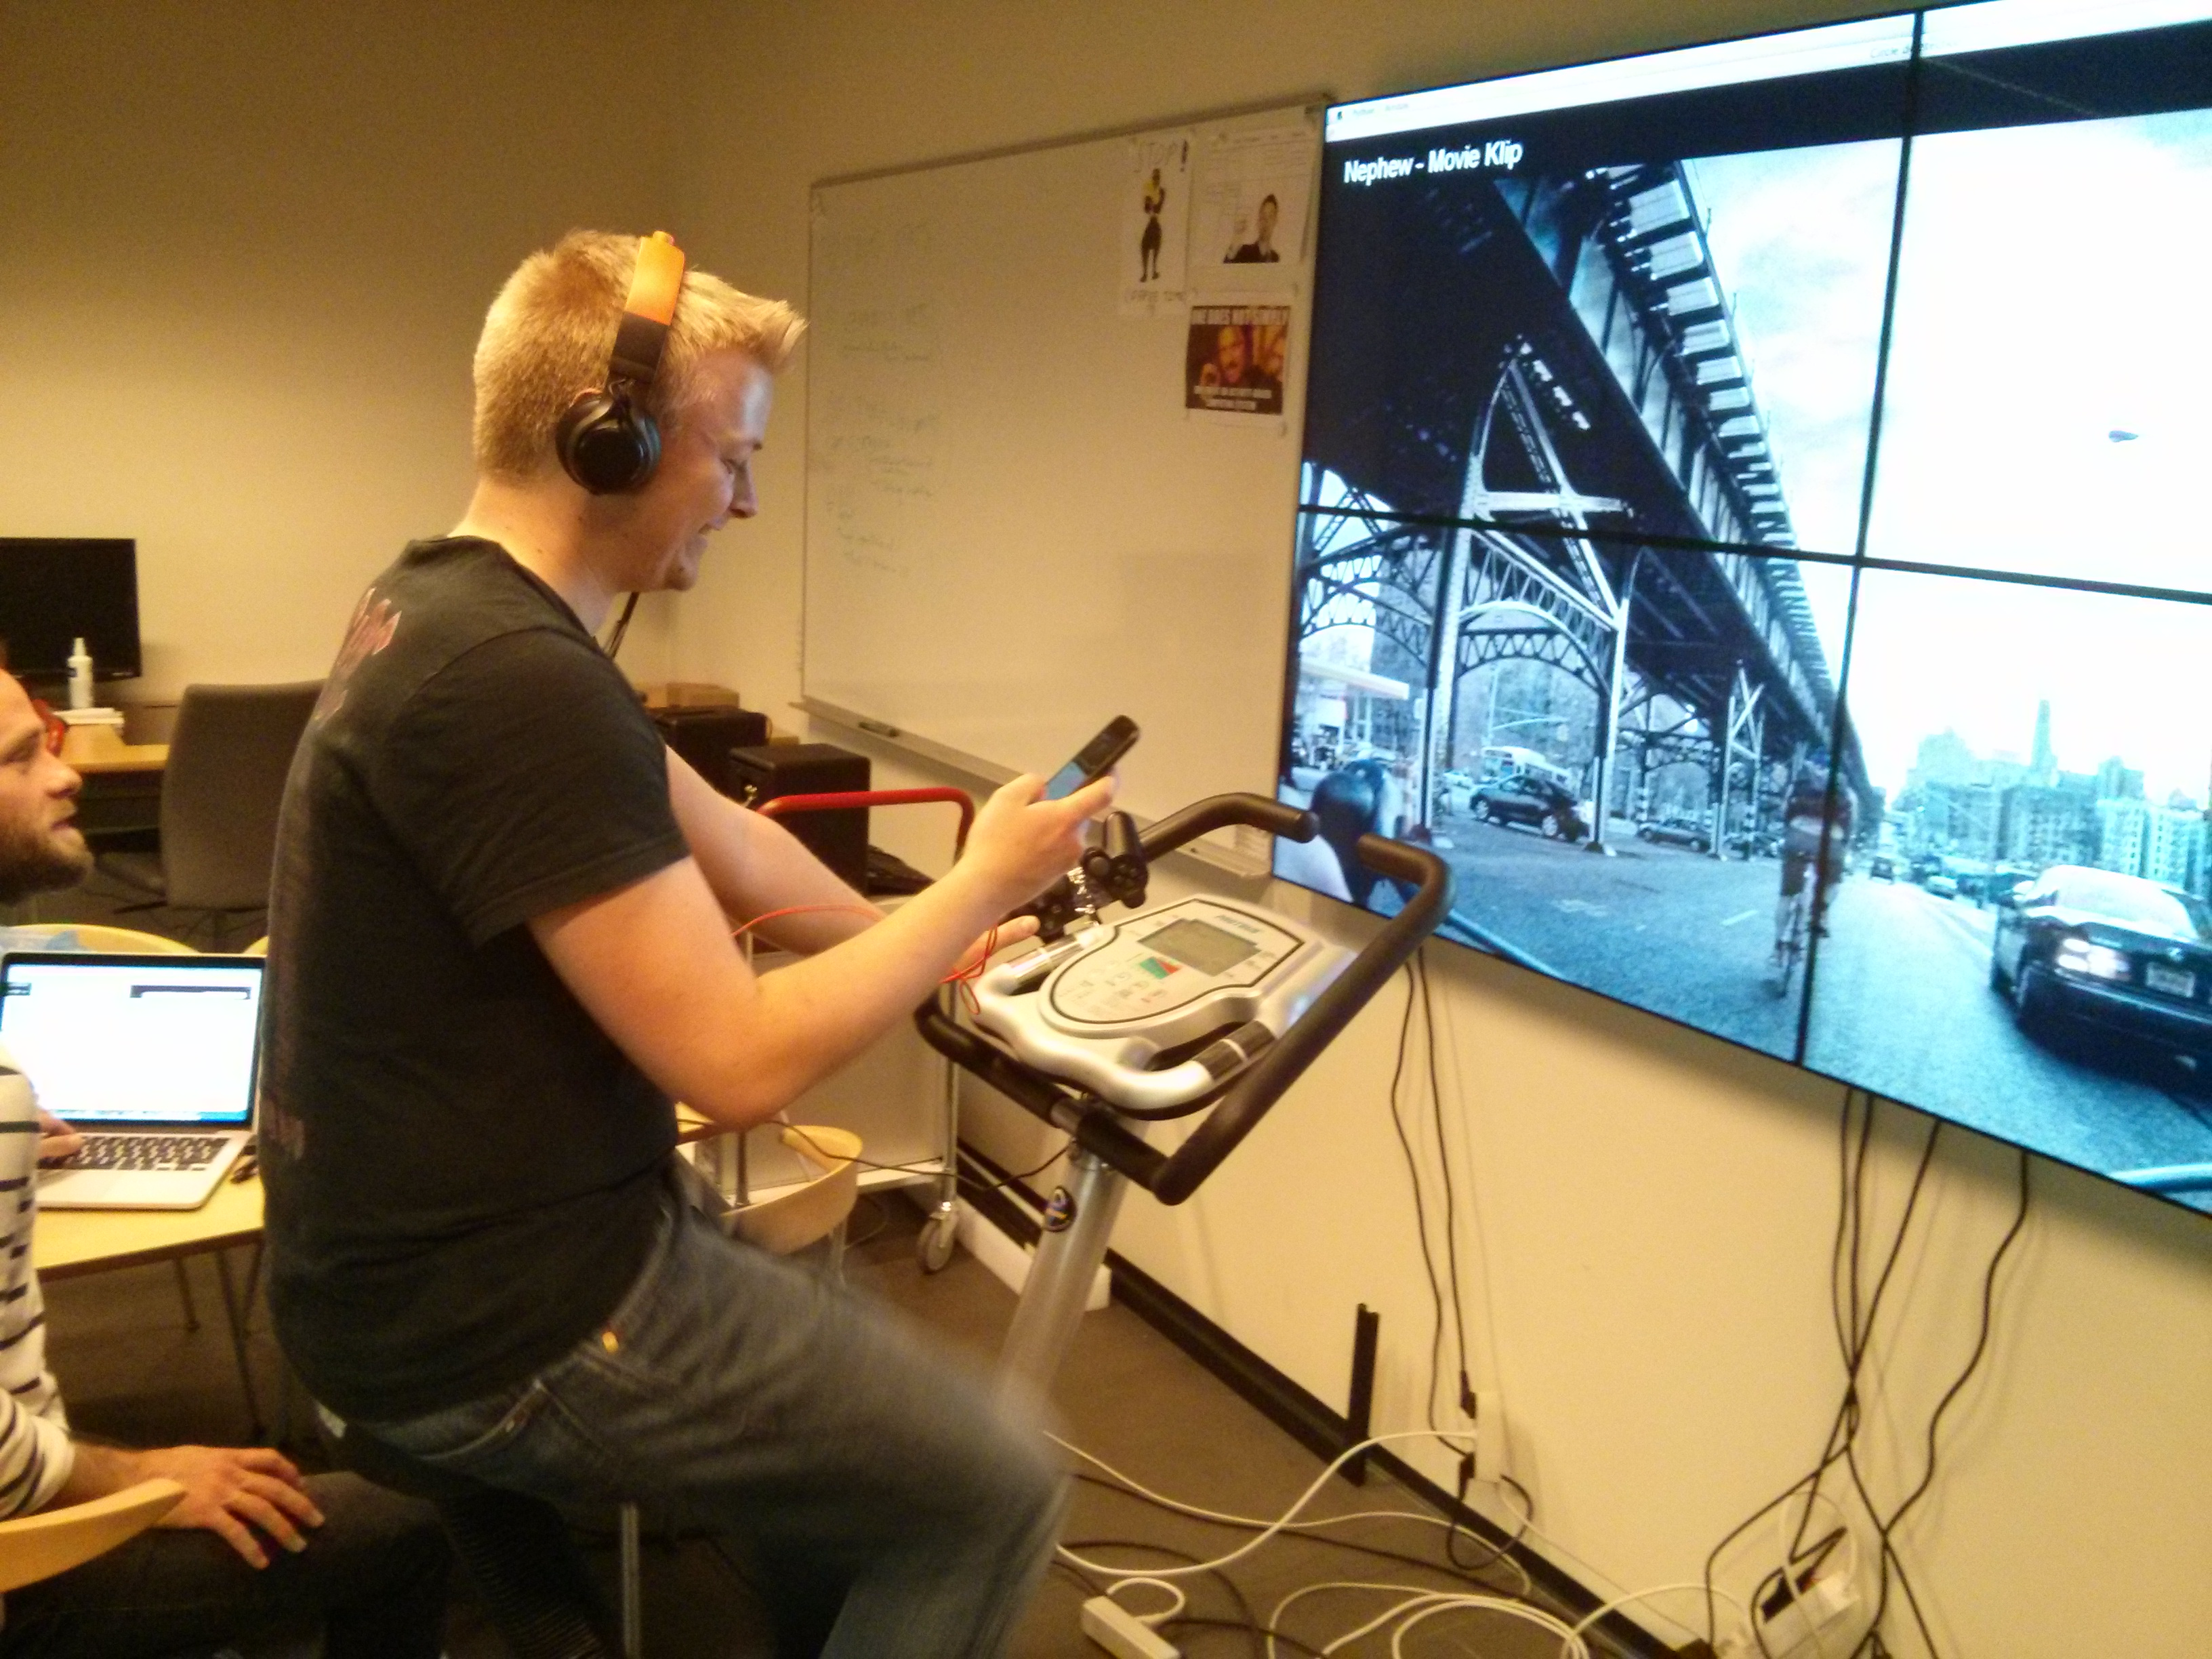
\includegraphics[width=0.7\textwidth,height=\textheight,keepaspectratio]{./Figures/evaluation_normal.jpg}
		\rule{35em}{1pt}
	\caption[Evaluation touch and vision-based interface]{Participant performing a task using a touch and vision-based music player}
	\label{fig:evalnormal}
\end{figure}

\subsection{Logging}
Throughout the experiment several data were logged. This includes data from the Biking Simulation System: Task start/end, circles shown, circles detections, error detections - and data from the Spatial Music Menu: Gestures detected, navigation steps including track info, headset connection status. Every log subject has a timestamp and as logging was performed on two different systems - iOS and OSX (python script) clocks were synchronized before comparison.


\subsection{NASA Task Load Index}
Subjective workload was measured using the NASA Task Load Index (TLX) scales \cite{hart_workload_1990}. The scales includes mental demand, physical demand, temporal demand, performance, effort and frustration in which each participant should rate after testing (Appendix \ref{sec:appendixnasatlx}). The user ratings gives a qualitative analysis of the system and the perceived workload is linked with the general usability of the system.

\subsection{Observation}
Participants were observed during the experiment to make sure they followed the instructions and to check and possibly prevent any kind of system obstruction. For example in between navigation tasks, when the user were listening to a selected track (PLAYING TRACK level), we made sure that the gyroscope was calibrated properly by compairing the direction on the iPad screen and the actual users head direction (using the calibrate button if neccesary, explained in \ref{sec:implementationviewsandcontrollers}). Also this observation gave us a chance to notice any particular repeating patterns in the way the users interacting with the systems, though we will not conclude anything from this in the results.


\section{Results}
This section presents the results of the experiment which were collected from logged data and the NASA TLX scales. Each participant did 9 tasks each, that is 45 tasks in total for each system and each participant filled out the NASA TLX scales for both systems.

\subsection{User attention}
We measured circle detection rate as an indicator of the users ability to attend to surroundings while interacting. The circle detection rate is the circles detected out of the circles shown during one task (in percent). Figure \ref{fig:resultscircles} shows the average rate for all 9 tasks for each participant using both systems.

\begin{figure}[h]
	\centering
		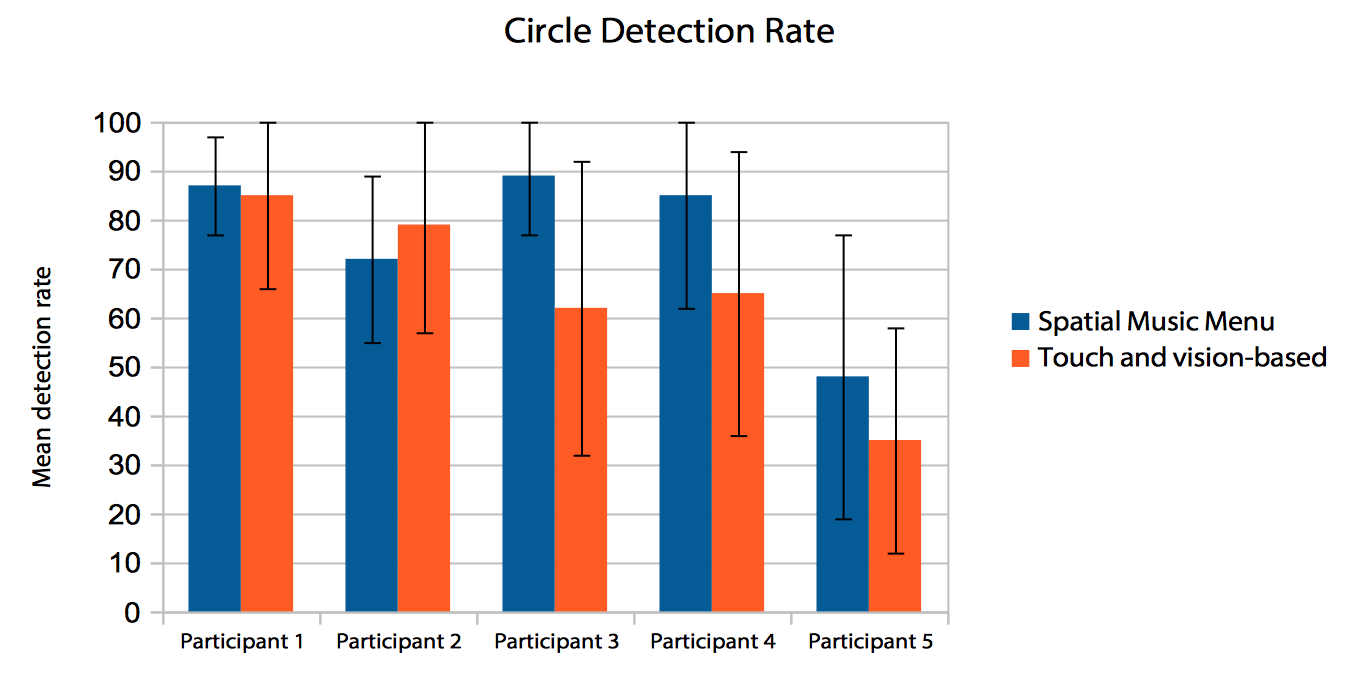
\includegraphics[width=0.9\textwidth,height=\textheight,keepaspectratio]{./Figures/results_circledetections.png}
		\rule{35em}{1pt}
	\caption[Results Circle Detection Rate]{Average circle detection rate for each participant}
	\label{fig:resultscircles}
\end{figure}

To verify \textit{Hypothesis 1} (page \pageref{sec:evaluationhypothesis}) we used a t-test to compaire circle detection rate between the two systems. The statistical test showed that there was a significant difference in the scores for the Spatial Music Menu (M=0.76) and the touch and vision-based music player (M=0.65) conditions; t(88)=1.66, p = 0.028 $<$ 0.05. In other words the circle detection rate is significantly higher when interacting with the Spatial Music Menu while biking.

\subsection{User performance}
Two measurements should give indications of the user performance. The first one is the task completion time - simply the time it took for a user to complete one task. Figure \ref{fig:resultstasktime} shows the average task completion time for all 9 tasks for each participant using both systems.

\begin{figure}[h]
	\centering
		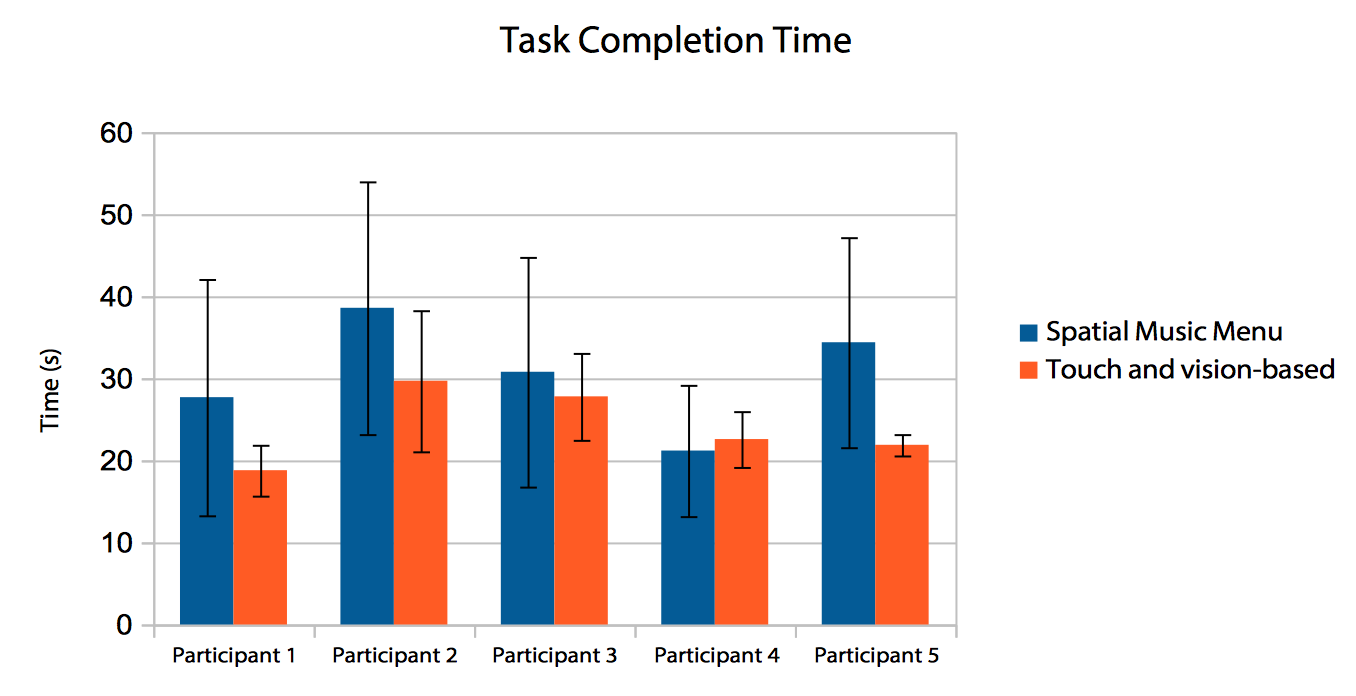
\includegraphics[width=0.9\textwidth,height=\textheight,keepaspectratio]{./Figures/results_tasktime.png}
		\rule{35em}{1pt}
	\caption[Results task time]{Time taken (in seconds) in average to execute a task for the participants.}
	\label{fig:resultstasktime}
\end{figure}

To verify \textit{Hypothesis 2} (page \pageref{sec:evaluationhypothesis}) in terms of task performance efficiency we used again a t-test to compaire the task completion time between the two systems. The statistical test showed that there was a significant difference in the scores for the Spatial Music Menu (M=30.53) and the touch and vision-based music player (M=24.13) conditions; t(88)=1.66, p = 0.003 $<$ 0.05. So in short the time it takes to complete a task, or navigate to a music track, is significantly higher in the Spatial Music Menu compaired to the touch and vision-based system.

To verify \textit{Hypothesis 2} in terms of the systems general usability we gathered qualitative data in form of participant ratings from the NASA TLX scales. The average of the participants scores for each of the 6 subscales are shown in figure \ref{fig:resultsnasatlx}.

\begin{figure}[h]
	\centering
		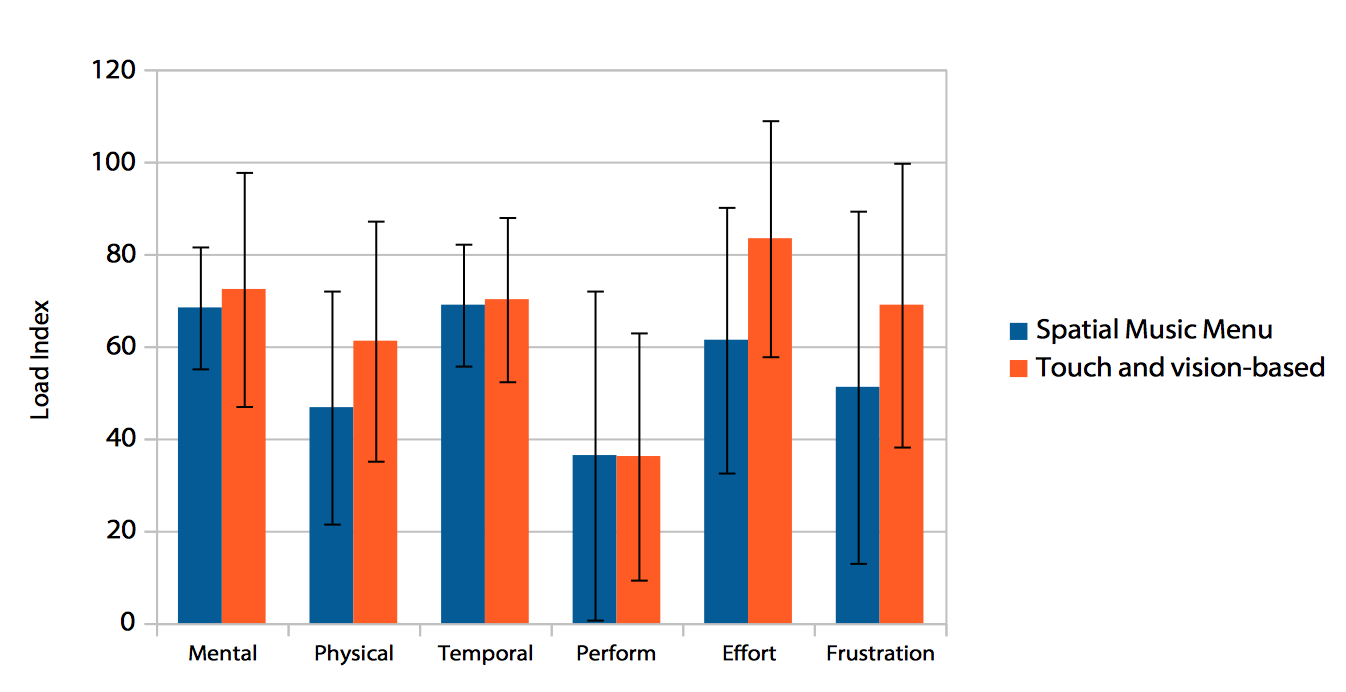
\includegraphics[width=0.9\textwidth,height=\textheight,keepaspectratio]{./Figures/results_taskloadindex.png}
		\rule{35em}{1pt}
	\caption[Results NASA TLX Score]{NASA TLX overall workload score for the participants (lower is better).}
	\label{fig:resultsnasatlx}
\end{figure}

The results show lower scores for the Spatial Music Menu in Physical Demand, Effort and Frustration while Mental Demand, Temporal Demand and Performance scores are more or less the same for both systems. The average of the participants total workload was 55.5 for the Spatial Music Menu and 65.4 for the touch and vision-based system.


\section{Discussion}
The results from the evaulation verified the first hypothesis, that participants were able to detect more circles interacting with the Spatial Music Menu comparied to the touch and vision-based. The main reason for this is that the visual focus can stay only on the screen (road) using the Spatial Music Menu while it is attending two visual tasks with the touch and vision-based system. It should be noted however that some participants during some tasks actually moved the eyes in the direction their head was pointing - however the chance of detecting a circle in the corner of the eye is still greater than when looking down on a screen.

The verification of the second hypothesis had mixed results. The task completion time for the Spatial Music Menu were significantly slower than the touch and vision-based system i.e. in terms of task performance efficiency the Spatial Music Menu could not compete with the touch and vision-based music player. If we look at figure \ref{fig:resultscircles} we notice a high spread for the Spatial Music Menu while the touch and vision-based system generally has a lower one making it more stable. However while the Spatial Music Menu shows that there exists challenges in that some tasks took a very long time to complete, it also shows a potential in that tasks can be performed very fast - faster than the touch and vision-based system.

However in terms of usability the Spatial Music Menu showed an overall lower workload score than the touch and vision-based music player. We are aware that these scores are only qualitative indications and that more than 5 participants could provide us with a more realistic picture.

\subsection{Challenges}
During the evaluation we observed a few challenges that could affect the results. First of all the headset gyroscope was a bit challenging in that it sometimes during execution of tasks "drifted" i.e. causing the menus center position moved a bit to the left/right. We did our best to calibrate the gyroscope in between tasks but this could affect a users task performance and workload.

Secondly some of the participants complained about some music tracks being higher in volume than others. This is due to the fact that the quality of music tracks provided by the Deezer music service variate.

TODO: shuffling tracks in spatial musicmenu maybe a greater challenge than the $>$ 3 album tracks, user can still create a virtual map

TODO: Spatial sound through headphones depend on the HRTF recorded and might not fit to all persons as the ear constructions are different (Brewster chapter 12 "Non-Speech Auditory Output" \cite{brewster_human-computer_2003})












% OLD
% Number of circles, safety
%The most important task for the user during testing is to detect as many circles as possible. The number of circles shown and the number of circles detected were logged during execution of tasks. This will give a quantitative analysis of whether the user is able to monitor the surroundings while interacting with the systems and contribute to the safety problem focus.

% System, track exploring
%For measuring the content (music track) exploring part of the Spatial Music Menu all navigation information were logged on the iPad. 

% System, task time

% Music genre type and quality made an impact

% the shuffling in the Spatial Music Menu is maybe making a to big difference (time), the user can still "map" tracks in the Deezer app though > 3 tracks. At the same time this enforces the spatial effect.

% Maybe comfort as a measurement?
%(Taken from Brewster article)
%The final measure taken was comfort. This was based around a new scale developed by Knight et al. [10] called the Comfort Rating Scale (CRS) which assesses various aspects to do with the comfort of a wearable device. For a device to be accepted and used it needs to be comfortable and people need to be happy to wear it. Using a range of 20- point rating scales similar to NASA TLX, CRS breaks com- fort into 6 categories: emotion, attachment, harm, perceived change, movement and anxiety. Knight et al. have used it to assess the comfort of two wearable devices they are building in their research group. Using this will allow us to find out more about the actual acceptability our systems.



